\documentclass[11pt,a4paper]{article}
\usepackage[utf8]{inputenc}
\usepackage[spanish]{babel}
\usepackage{graphicx}
\usepackage{geometry}
\usepackage{hyperref}
\usepackage{float}
\usepackage[section]{placeins}  % Evita que floats se muevan a otras secciones
\usepackage{flafter}  % Fuerza que floats aparezcan después de ser referenciados
\usepackage{amsmath}
\usepackage{booktabs}
\usepackage{caption}
\usepackage{subcaption}
\usepackage{setspace}  % Para controlar interlineado

% Configuración de espaciado
\setstretch{1.15}  % Interlineado 1.15 (un poco más que simple)
\setlength{\parskip}{0.4em}  % Espacio entre párrafos
\setlength{\parindent}{1.5em}  % Sangría en primera línea

\geometry{margin=2.5cm}

% Mejores prácticas para control de flotantes
\setlength{\textfloatsep}{10pt plus 2pt minus 2pt}
\setlength{\floatsep}{10pt plus 2pt minus 2pt}
\setlength{\intextsep}{10pt plus 2pt minus 2pt}
\renewcommand{\topfraction}{0.9}
\renewcommand{\bottomfraction}{0.8}
\renewcommand{\textfraction}{0.1}
\renewcommand{\floatpagefraction}{0.7}

\hypersetup{
    colorlinks=true,
    linkcolor=blue,
    urlcolor=blue,
    citecolor=blue
}

\title{\textbf{Trabajo Práctico N° 1}}
\author{
    Juan Ignacio Pintos, Luis Mella, Paula Leylén Ramírez \\
    Taller de Programación, Universidad de Buenos Aires    
}
\date{Octubre 2025}

\begin{document}

\maketitle

\noindent\textbf{Repositorio GitHub:} \url{https://github.com/paulaleylen/BigDataUBA-GrupoJLP}

\section{Introducción}

El presente trabajo tiene como objetivo familiarizarnos con la Encuesta Permanente de Hogares (EPH) del INDEC, una herramienta fundamental para el estudio de la estructura socioeconómica argentina. A través del análisis comparativo entre el primer trimestre de 2005 y 2025 para la región del Gran Buenos Aires, buscamos identificar patrones en la evolución de la pobreza, las características demográficas y las condiciones de vida de la población.

La EPH es un programa nacional de producción sistemática de indicadores sociales que permite conocer características sociodemográficas y socioeconómicas de la población argentina. Para este estudio, trabajamos con microdatos individuales y de hogares, aplicando procesos de limpieza, transformación y análisis exploratorio de datos.

\section{Parte I: Familiarización con la base EPH y limpieza}

El INDEC utiliza el método del ingreso para medir la pobreza, basándose en la Canasta Básica Total (CBT). Una persona es considerada pobre cuando el ingreso total familiar del hogar al que pertenece no alcanza para cubrir el valor de dicha canasta. La metodología considera tres componentes: el Ingreso Total Familiar (ITF), que incluye todas las fuentes de ingreso monetario del hogar; la Canasta Básica Total por adulto equivalente, que incorpora alimentos y bienes no alimentarios (vestimenta, transporte, educación, vivienda); y el concepto de adulto equivalente, que pondera las necesidades energéticas según sexo y edad (un varón adulto equivale a 1.0, un niño de 2 años a 0.46). La línea de pobreza se define como el producto de la CBT por adulto equivalente multiplicado por la cantidad total de adultos equivalentes del hogar. Si el ITF es inferior a este valor, todos los miembros del hogar son clasificados como pobres.

Para este estudio seleccionamos la región Gran Buenos Aires (GBA), que concentra aproximadamente un tercio de la población argentina y representa el principal polo económico del país. Las bases de datos incluyen 9,484 observaciones individuales para 2005 (formato Stata .dta) y 7,181 para 2025 (formato Excel .xls), totalizando 16,665 observaciones tras filtrado regional y concatenación. Los datos presentan diferencias estructurales significativas: en 2005 las variables categóricas se codifican con texto descriptivo (``Gran Buenos Aires''), mientras que en 2025 se utiliza codificación numérica (código 1 para GBA, 40-44 para otras regiones), requiriendo estandarización mediante mapeos de equivalencias.

La reducción del 24.3\% en el tamaño muestral entre ambos períodos merece atención. Esta contracción podría reflejar desafíos operativos del INDEC en 2025: mayores tasas de rechazo al relevamiento, dificultades de acceso a hogares vulnerables, o ajustes en el diseño muestral. Combinada con la alta tasa de no respuesta en variables de ingreso, podría estar afectando la precisión de las estimaciones de pobreza para el período más reciente.

Seleccionamos 16 variables: las obligatorias (CH04, CH06, CH07, CH08, NIVEL\_ED, ESTADO, CAT\_INAC, IPCF) y otras relevantes (ITF, P21, CAT\_OCUP, PP03J). El análisis de valores faltantes (Figura \ref{fig:missing}, ver Apéndice) muestra que en 2005 no hay valores faltantes en el formato original, pues el INDEC usaba códigos especiales ($-9$, $-1$) para no respuesta. En 2025, la variable PP03J presenta 52.68\% de valores faltantes, patrón estructuralmente correcto ya que desocupados e inactivos no reportan horas trabajadas.

El proceso de limpieza convirtió a NA los códigos $-9$ (``No sabe / No responde'') y $-1$ (``No responde / No corresponde'') en CH06 (42 valores) y P21 (919 valores). El código 0 se mantuvo válido, representando ausencia legítima de ingresos.

Como ejercicio adicional, realizamos cuatro tipos de uniones entre las bases de individuos y hogares (2005 y 2025) utilizando las claves CODUSU y NRO\_HOGAR. La Tabla \ref{tab:joins} presenta los resultados.

\begin{table}[H]
\centering
\begin{tabular}{lccc}
\toprule
\textbf{Tipo de unión} & \textbf{Nro. de filas} & \textbf{Nro. de columnas} & \textbf{Total de NAs} \\
\midrule
Intersección (inner) & 16,665 & 21 & 4,879 \\
Izquierda (left) & 16,665 & 21 & 4,879 \\
Derecha (right) & 16,665 & 21 & 4,879 \\
Conjunta (outer) & 16,665 & 21 & 4,879 \\
\bottomrule
\end{tabular}
\caption{Resultados de la unión entre bases de Individuos y Hogares de la EPH}
\label{tab:joins}
\end{table}

La coincidencia perfecta en las cuatro operaciones de unión (mismo número de filas, columnas y valores faltantes) indica que existe correspondencia total entre las observaciones: cada individuo tiene exactamente un hogar asociado y viceversa. Esto valida la integridad referencial de las bases de datos del INDEC y garantiza que no existen registros huérfanos en ninguna de las dos tablas.

\section{Parte II: Primer Análisis Exploratorio}

La distribución por sexo (Figura \ref{fig:sexo}, ver Apéndice) muestra una inversión demográfica notable. En 2005 hay leve mayoría masculina (52.51\% varones vs 47.49\% mujeres), mientras que en 2025 se invierte con mayoría femenina (52.11\% mujeres vs 47.89\% varones). Este cambio de 5 puntos porcentuales sugiere feminización gradual del GBA, coherente con tendencias urbanas latinoamericanas. El fenómeno puede atribuirse a diferencias en esperanza de vida por sexo (mujeres viven 6-7 años más), variaciones en patrones migratorios internos (mujeres jóvenes migrando al GBA por oportunidades educativas/laborales en servicios), y posibles sesgos de muestreo (mayor disponibilidad femenina durante relevamientos).

Las matrices de correlación (Figuras \ref{fig:corr2005} y \ref{fig:corr2025}, ver Apéndice) incorporan variables dummy para categóricas, generando 36 variables para 2005 y 34 para 2025. Las correlaciones más significativas en 2025 incluyen: Inactividad-Estudiante vs Educación-Primaria ($r = 0.91$), Estado civil Viudo vs Unido ($r = -0.84$), y Actividad-Ocupado vs Actividad-Desocupado ($r = -0.75$). Comparando períodos, la correlación entre educación universitaria y ocupación aumentó de $r = 0.45$ (2005) a $r = 0.61$ (2025), sugiriendo que la educación se volvió determinante más crítico del acceso laboral formal. Sin embargo, las correlaciones entre ingresos (IPCF, ITF) y educación se debilitaron, indicando que la educación facilita acceso al empleo pero no garantiza ingresos suficientes para escapar de la pobreza. Esta desconexión entre credenciales educativas y seguridad económica señala una crisis de retornos a la educación en contexto de deterioro económico generalizado.

\section{Parte III: Conociendo a los pobres y no pobres}

Uno de los hallazgos más preocupantes del análisis es el dramático incremento de hogares declarando ingresos nulos. En 2005, apenas el 1.2\% de las observaciones (113 casos) reportaron ITF igual a cero (sin ingresos monetarios). Para 2025, esta cifra se disparó al 40.0\% (2,872 casos), multiplicándose por 33 en dos décadas. Si bien ITF=0 es técnicamente un valor válido que representa hogares sin ingresos monetarios, su magnitud en 2025 plantea serios interrogantes sobre la calidad de los datos y la representatividad de los resultados. Este fenómeno puede reflejar tanto una crisis económica real (informalidad extrema, desempleo) como problemas de recolección de datos (renuencia a declarar ingresos informales). La literatura del INDEC documenta que la no declaración de ingresos no es aleatoria: típicamente, hogares de muy altos ingresos subreportan por desconfianza, mientras hogares en extrema precariedad no declaran ingresos informales, generando un doble sesgo que complica las estimaciones de pobreza.

Utilizando la tabla de adulto equivalente provista, que pondera las necesidades energéticas por sexo y edad, calculamos el adulto equivalente individual según edad y sexo (rango: 0.35 para menores de 1 año hasta 1.06 para varones adultos), y la suma de adultos equivalentes por hogar mediante agrupación por identificador de hogar. La línea de pobreza (INGRESO\_NECESARIO) se define como el producto de la CBT por adulto equivalente multiplicado por la cantidad total de adultos equivalentes del hogar, donde la Canasta Básica Total (CBT) es de \$205.07 para 2005 y \$365,177 para 2025. La magnitud de la inflación implícita (aproximadamente 178,000\% en 20 años) refleja la profunda crisis macroeconómica argentina del período.

Clasificamos como pobre a toda persona cuyo hogar cumple ITF $<$ INGRESO\_NECESARIO. Los resultados son alarmantes: la pobreza pasó de 26.88\% en 2005 (2,564 de 9,538 personas) a 58.86\% en 2025 (4,259 de 7,236 personas), representando un incremento de 31.98 puntos porcentuales. La pobreza más que se duplicó en términos relativos, pasando de afectar a poco más de uno de cada cuatro habitantes del GBA a casi seis de cada diez. En términos absolutos, el número de pobres creció 66\% a pesar de la reducción del 24\% en el tamaño de la muestra. Este incremento representa una de las mayores expansiones de pobreza urbana registradas en Argentina en contextos no hiperinflacionarios.

El análisis descriptivo comparativo (Tabla \ref{tab:descriptivos}) revela patrones consistentes en ambos períodos: los pobres viven en hogares más grandes (4.33 vs 3.03 adultos equivalentes en 2005; 3.27 vs 2.49 en 2025), son más jóvenes en promedio (26.3 vs 37.6 años en 2005; 36.6 vs 41.4 años en 2025), y tienen ingresos per cápita significativamente menores (\$93 vs \$572 en 2005; \$58,210 vs \$820,653 en 2025). Sin embargo, la brecha absoluta de ingresos se amplió exponencialmente entre 2005 y 2025.

\begin{table}[H]
\centering
\small
\begin{tabular}{lcccc}
\toprule
 & \multicolumn{2}{c}{\textbf{2005}} & \multicolumn{2}{c}{\textbf{2025}} \\
\cmidrule(lr){2-3} \cmidrule(lr){4-5}
\textbf{Variable} & \textbf{Pobres} & \textbf{No Pobres} & \textbf{Pobres} & \textbf{No Pobres} \\
\midrule
Edad (media) & 26.25 & 37.63 & 36.55 & 41.40 \\
IPCF (media) & \$93.04 & \$572.23 & \$58,210 & \$820,653 \\
ITF (media) & \$505 & \$1,884 & \$239,479 & \$2,302,636 \\
Ad. equiv. hogar & 4.33 & 3.03 & 3.27 & 2.49 \\
Observaciones & 2,564 & 6,974 & 4,259 & 2,977 \\
\bottomrule
\end{tabular}
\caption{Estadísticas descriptivas: pobres vs no pobres por año}
\label{tab:descriptivos}
\end{table}

La distribución de ingresos (Figura \ref{fig:ipcf}, ver Apéndice) revela cambios dramáticos. En 2005, ambas distribuciones eran compactas con outliers moderados: pobres mostraban IPCF mediano de \$80, no pobres de \$450 (brecha 5.6 veces). Para 2025, muchos pobres reportan IPCF cero (un cuarto de los pobres sin ingreso monetario declarado, indigencia absoluta), mientras no pobres muestran dispersión extrema con outliers superiores a \$10 millones mensuales per cápita. La brecha se amplió exponencialmente: en 2005 un no pobre ganaba 6.1 veces más que un pobre (\$572 vs \$93), en 2025 la brecha creció a 14.1 veces (\$820,653 vs \$58,210). Esta divergencia sugiere que los mecanismos tradicionales de movilidad social dejaron de funcionar como puentes entre estratos, consolidando una sociedad segmentada.

La composición de pobreza por nivel educativo (Figura \ref{fig:educacion}, ver Apéndice) evidencia el colapso de la educación como protección. En 2005, la pobreza se concentraba en niveles bajos y medios, con educación superior actuando como protección (tasas $<$10\% para universitarios completos). Para 2025, la pobreza afecta transversalmente todos los niveles, incluyendo universitarios completos (tasas 30-35\%). Este hallazgo indica crisis estructural: cuando la economía se contrae generalizadamente, ni las credenciales más altas garantizan seguridad económica. El problema no es de oferta de trabajo calificado sino de demanda de empleo de calidad.

\section{Conclusiones}

El análisis comparativo de la EPH entre 2005 y 2025 para el Gran Buenos Aires revela una profunda transformación de la estructura socioeconómica que trasciende las fluctuaciones cíclicas habituales de la economía argentina. La pobreza experimentó una explosión sin precedentes, pasando del 26.88\% al 58.86\%, convirtiendo a casi seis de cada diez habitantes del GBA en pobres. Este incremento de 31.98 puntos porcentuales en dos décadas representa una de las mayores expansiones de pobreza urbana registradas en América Latina en contextos no hiperinflacionarios, equiparable a crisis severas como la de Argentina en 2001-2002, pero sostenida en el tiempo.

La crisis de calidad de datos constituye un hallazgo alarmante en sí mismo. La tasa de no respuesta en ITF se multiplicó por 33, pasando de 1.2\% a 40.0\%. Esta erosión de la calidad de los datos no es un problema técnico menor: compromete la representatividad de los resultados y plantea desafíos metodológicos serios para el monitoreo de indicadores sociales. Si cuatro de cada diez hogares no reportan ingresos, las estimaciones de pobreza basadas en el 60\% restante pueden estar sesgadas de manera impredecible. La literatura especializada documenta que la no respuesta en encuestas de ingresos no es aleatoria: típicamente, los hogares de muy altos ingresos subreportan por desconfianza o evasión fiscal, mientras que los hogares en situación de precariedad extrema también pueden subreportar por informalidad completa. Este doble sesgo complica la interpretación de los resultados y exige cautela al formular políticas basadas en estos datos.

La polarización de ingresos se intensificó dramáticamente, con una sociedad cada vez más fragmentada. Mientras algunos hogares reportan ingresos per cápita superiores a \$10 millones mensuales (aproximadamente 27 veces el salario mínimo de 2025), una proporción creciente declara ingresos nulos o cercanos a cero. Esta divergencia extrema no solo refleja desigualdad de ingresos, sino desigualdad de oportunidades, de acceso a servicios, de capital social y de poder político. La desigualdad extrema erosiona la cohesión social, debilita la confianza en las instituciones y genera inestabilidad política, como documenta abundante evidencia internacional.

El colapso de la educación como mecanismo de protección contra la pobreza es quizás el hallazgo más inquietante del análisis. En 2005, la educación superior actuaba como un escudo robusto: completar la universidad prácticamente garantizaba escapar de la pobreza. Para 2025, universitarios completos enfrentan tasas de pobreza cercanas al 30-35\%, evidenciando una crisis que trasciende el capital humano individual. Cuando la educación pierde su capacidad de traducirse en seguridad económica, se erosiona uno de los pilares fundamentales de la movilidad social y se deslegitiman los discursos meritocráticos tradicionales. Este fenómeno sugiere que el problema no es de oferta de trabajo calificado (Argentina tiene tasas relativamente altas de educación superior), sino de demanda de empleo de calidad: la economía no está generando suficientes puestos de trabajo bien remunerados para absorber a los trabajadores calificados.

Los hogares pobres mantienen características estructurales consistentes en ambos períodos: son más grandes (más adultos equivalentes por hogar), más jóvenes (menor edad promedio de sus miembros) y tienen menores ingresos per cápita. Sin embargo, estas características operan en un contexto macroeconómico radicalmente diferente que amplifica las vulnerabilidades. En 2005, un hogar pobre enfrentaba privaciones pero podía aspirar a movilidad ascendente mediante educación o migración hacia sectores formales. En 2025, esas escaleras de movilidad parecen haberse quebrado: incluso con educación superior, las probabilidades de escapar de la pobreza se han reducido drásticamente.

\section{Referencias}

\begin{itemize}
\item INDEC (2025). \textit{Encuesta Permanente de Hogares - Primer Trimestre 2025. Base de Microdatos.} Instituto Nacional de Estadística y Censos. Disponible en: \url{https://www.indec.gob.ar/indec/web/Institucional-Indec-BasesDeDatos}

\item INDEC (2005). \textit{Encuesta Permanente de Hogares - Primer Trimestre 2005. Base de Microdatos.} Instituto Nacional de Estadística y Censos.

\item INDEC (2024). \textit{Diseño de registro y estructura para las bases preliminares Hogar y Personas. EPH Continua.} Documento metodológico. Instituto Nacional de Estadística y Censos.

\end{itemize}

\newpage

\appendix

\section{Figuras complementarias}

\begin{figure}[htb!]
    \centering
    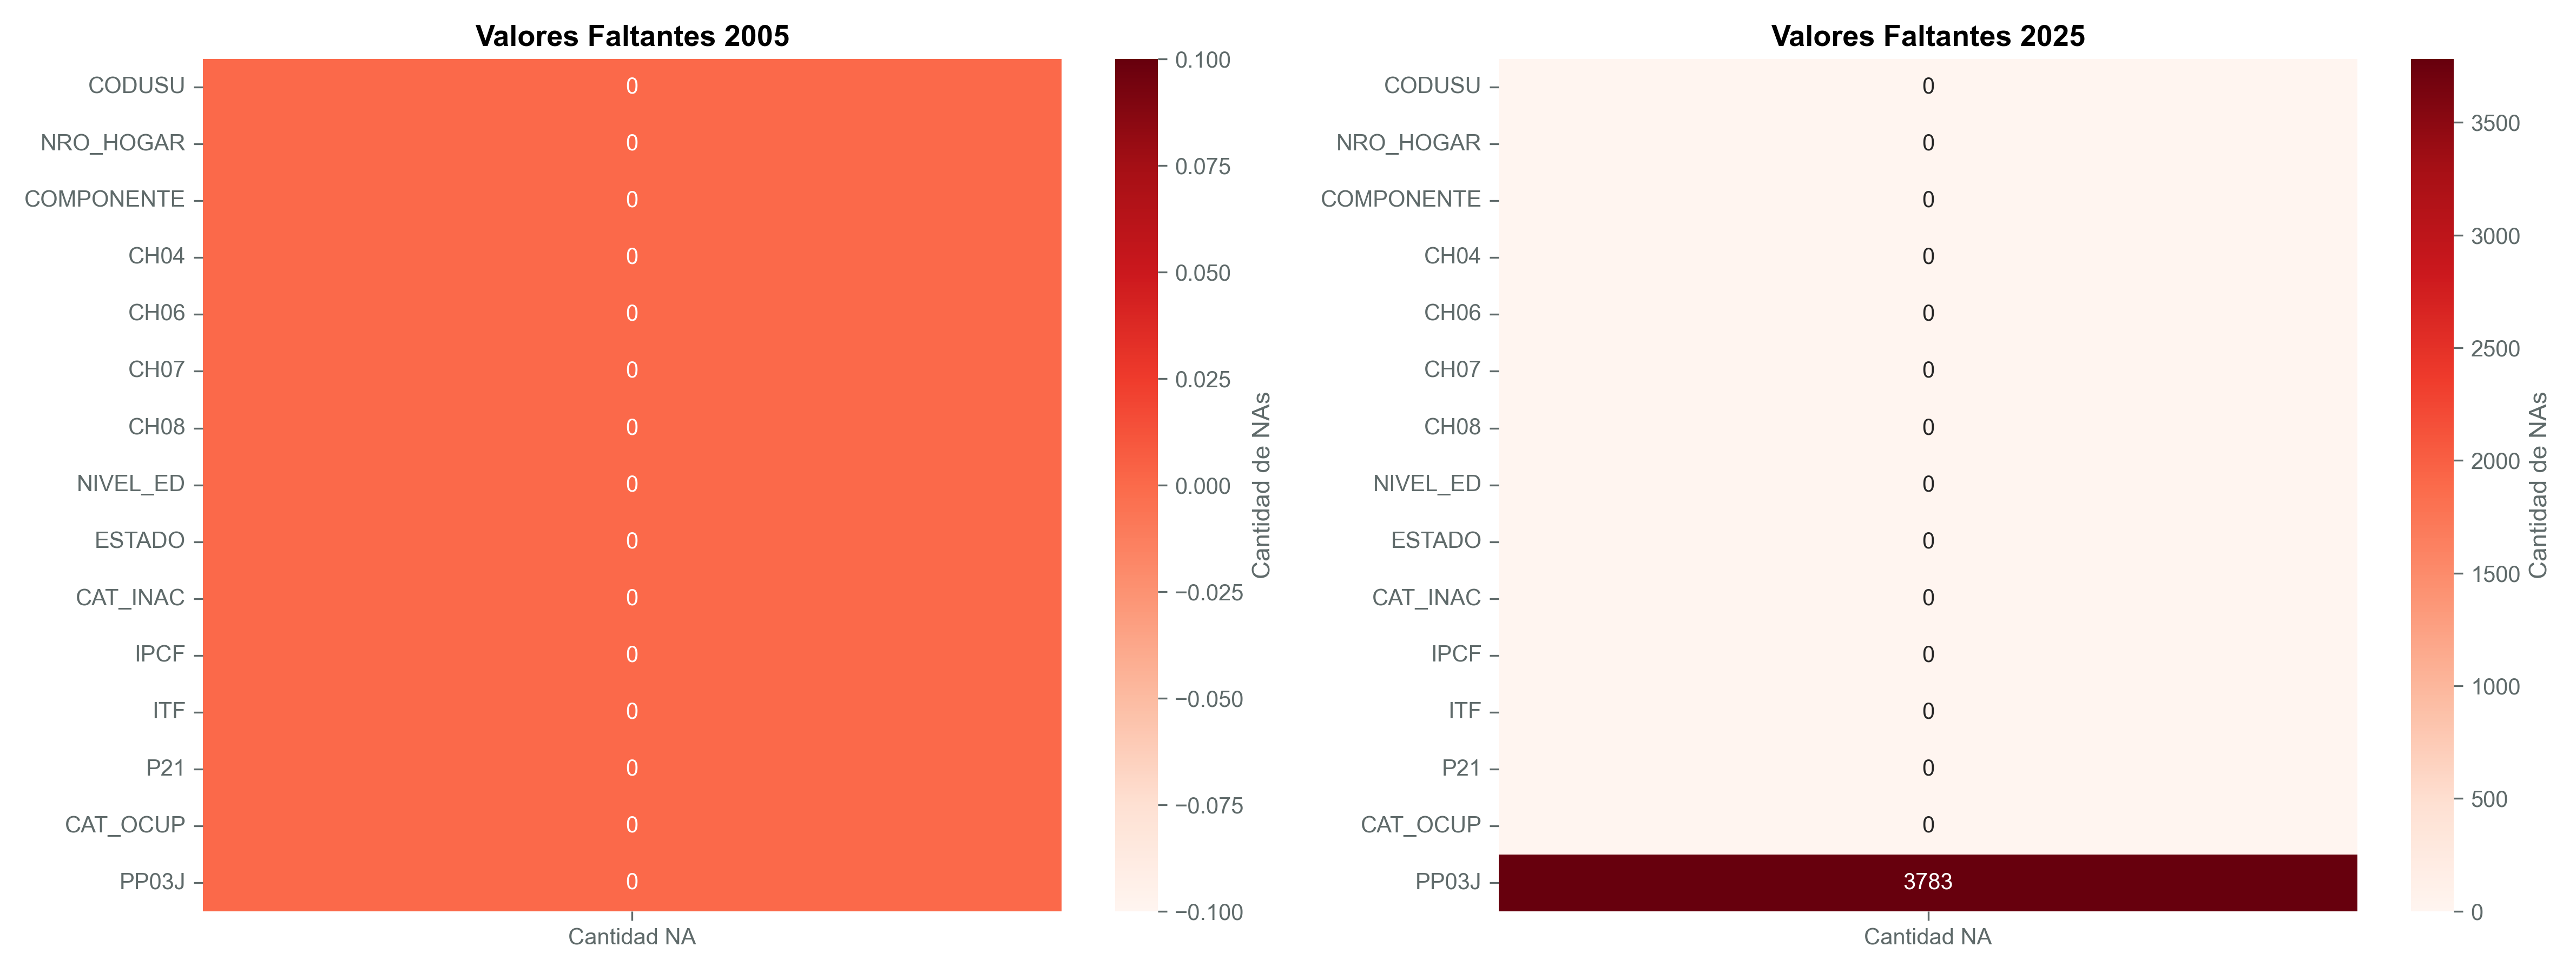
\includegraphics[width=1\textwidth]{../graficos/figura_missing_values.png}
    \caption{Valores faltantes por variable y año en Gran Buenos Aires}
    \label{fig:missing}
\end{figure}

\begin{figure}[htb!]
    \centering
    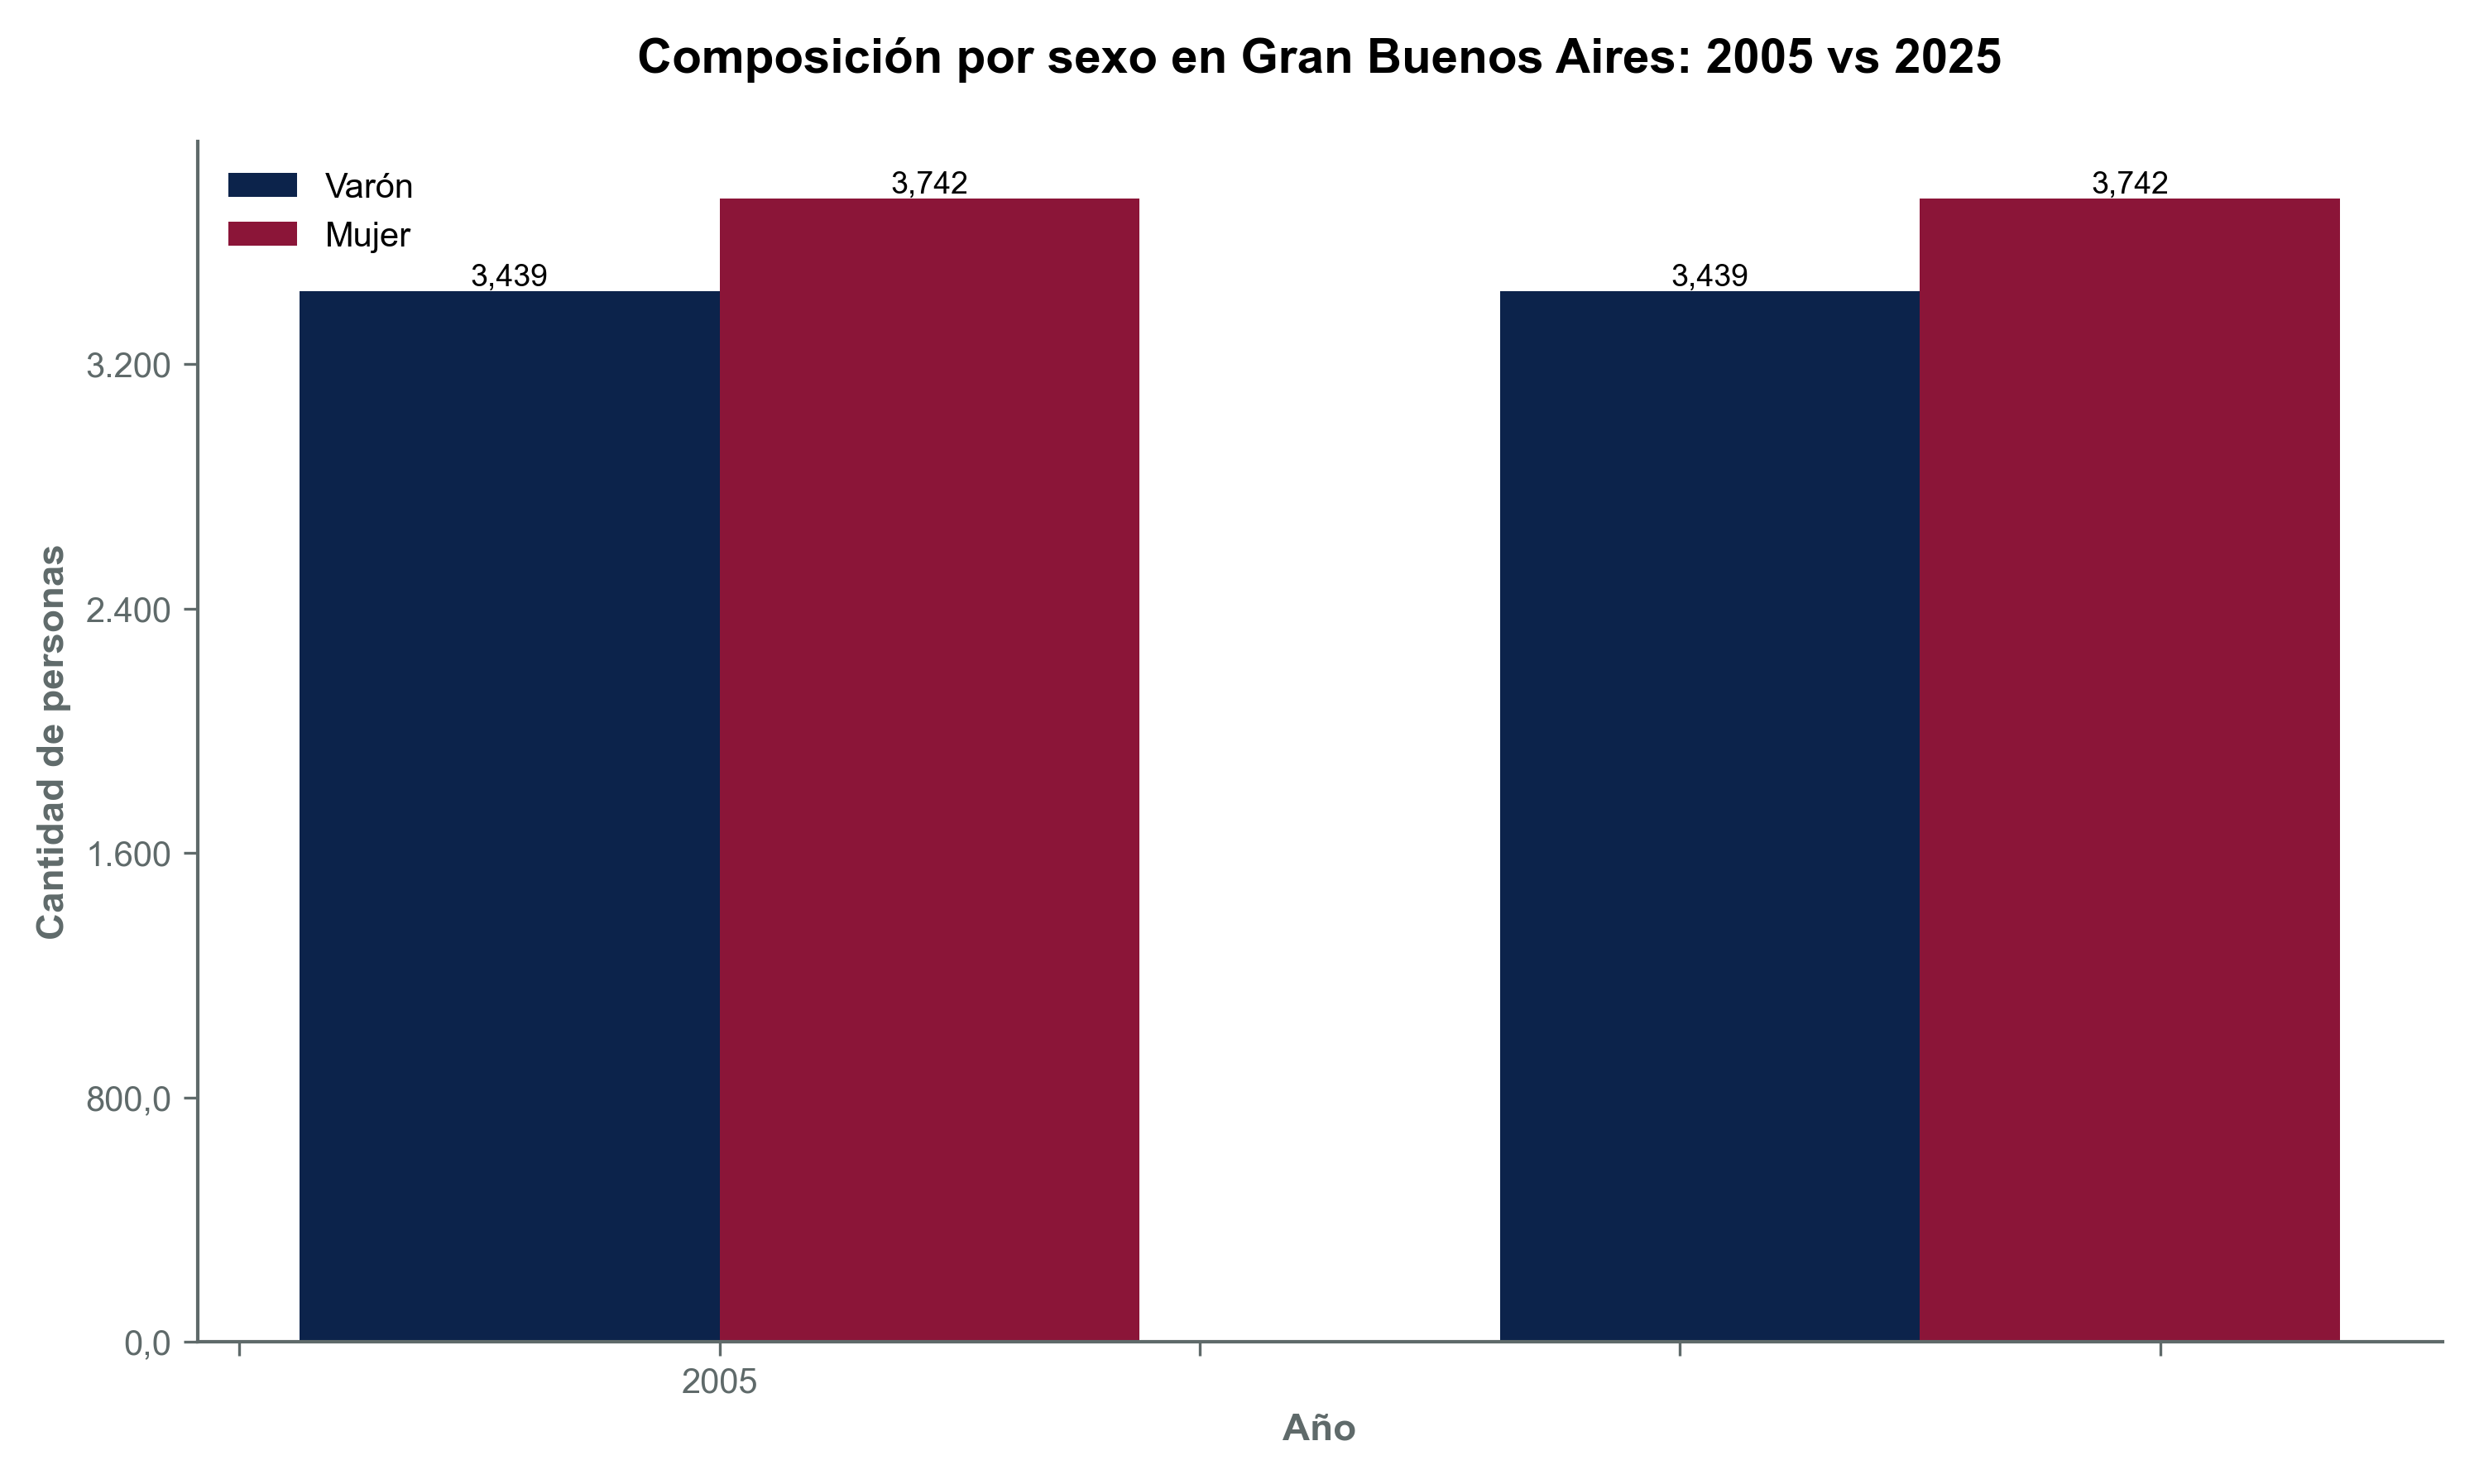
\includegraphics[width=1\textwidth]{../graficos/composicion_sexo_2005_2025.png}
    \caption{Composición por sexo en Gran Buenos Aires: comparación 2005-2025}
    \label{fig:sexo}
\end{figure}

\begin{figure}[htb!]
    \centering
    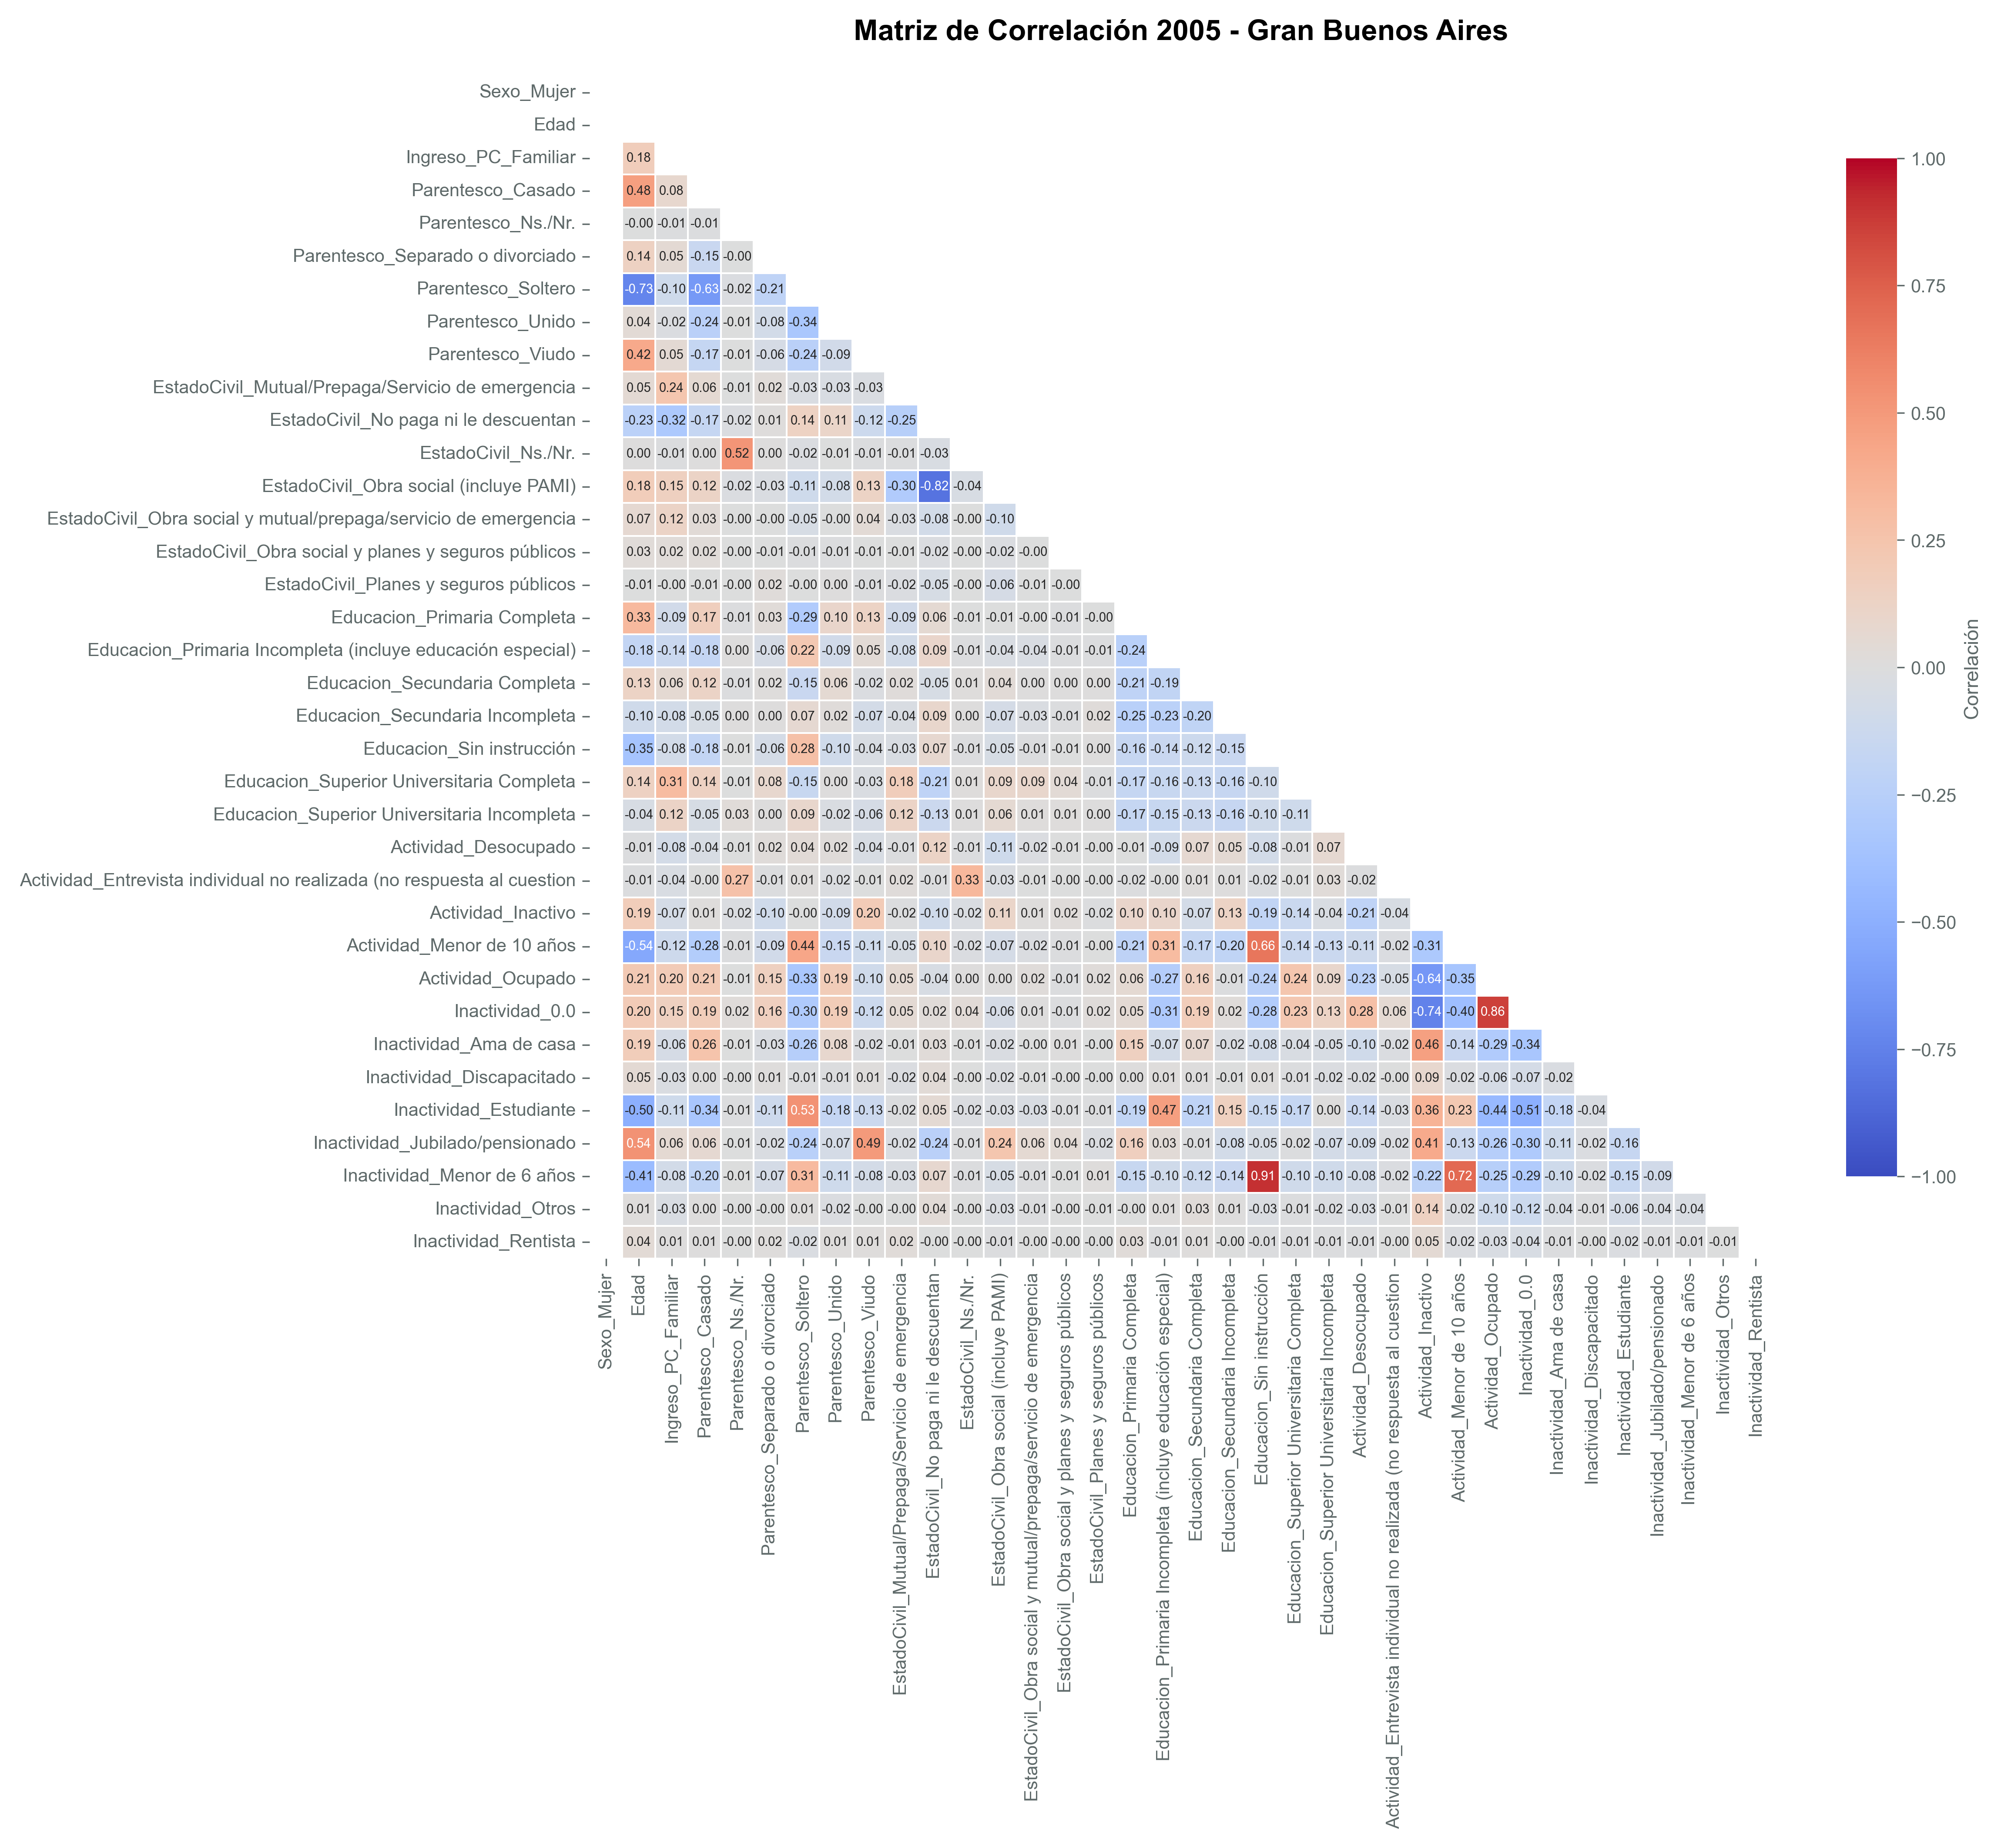
\includegraphics[width=0.8\textwidth]{../graficos/matriz_correlacion_2005.png}
    \caption{Matriz de correlación 2005 --- Gran Buenos Aires}
    \label{fig:corr2005}
\end{figure}

\begin{figure}[htb!]
    \centering
    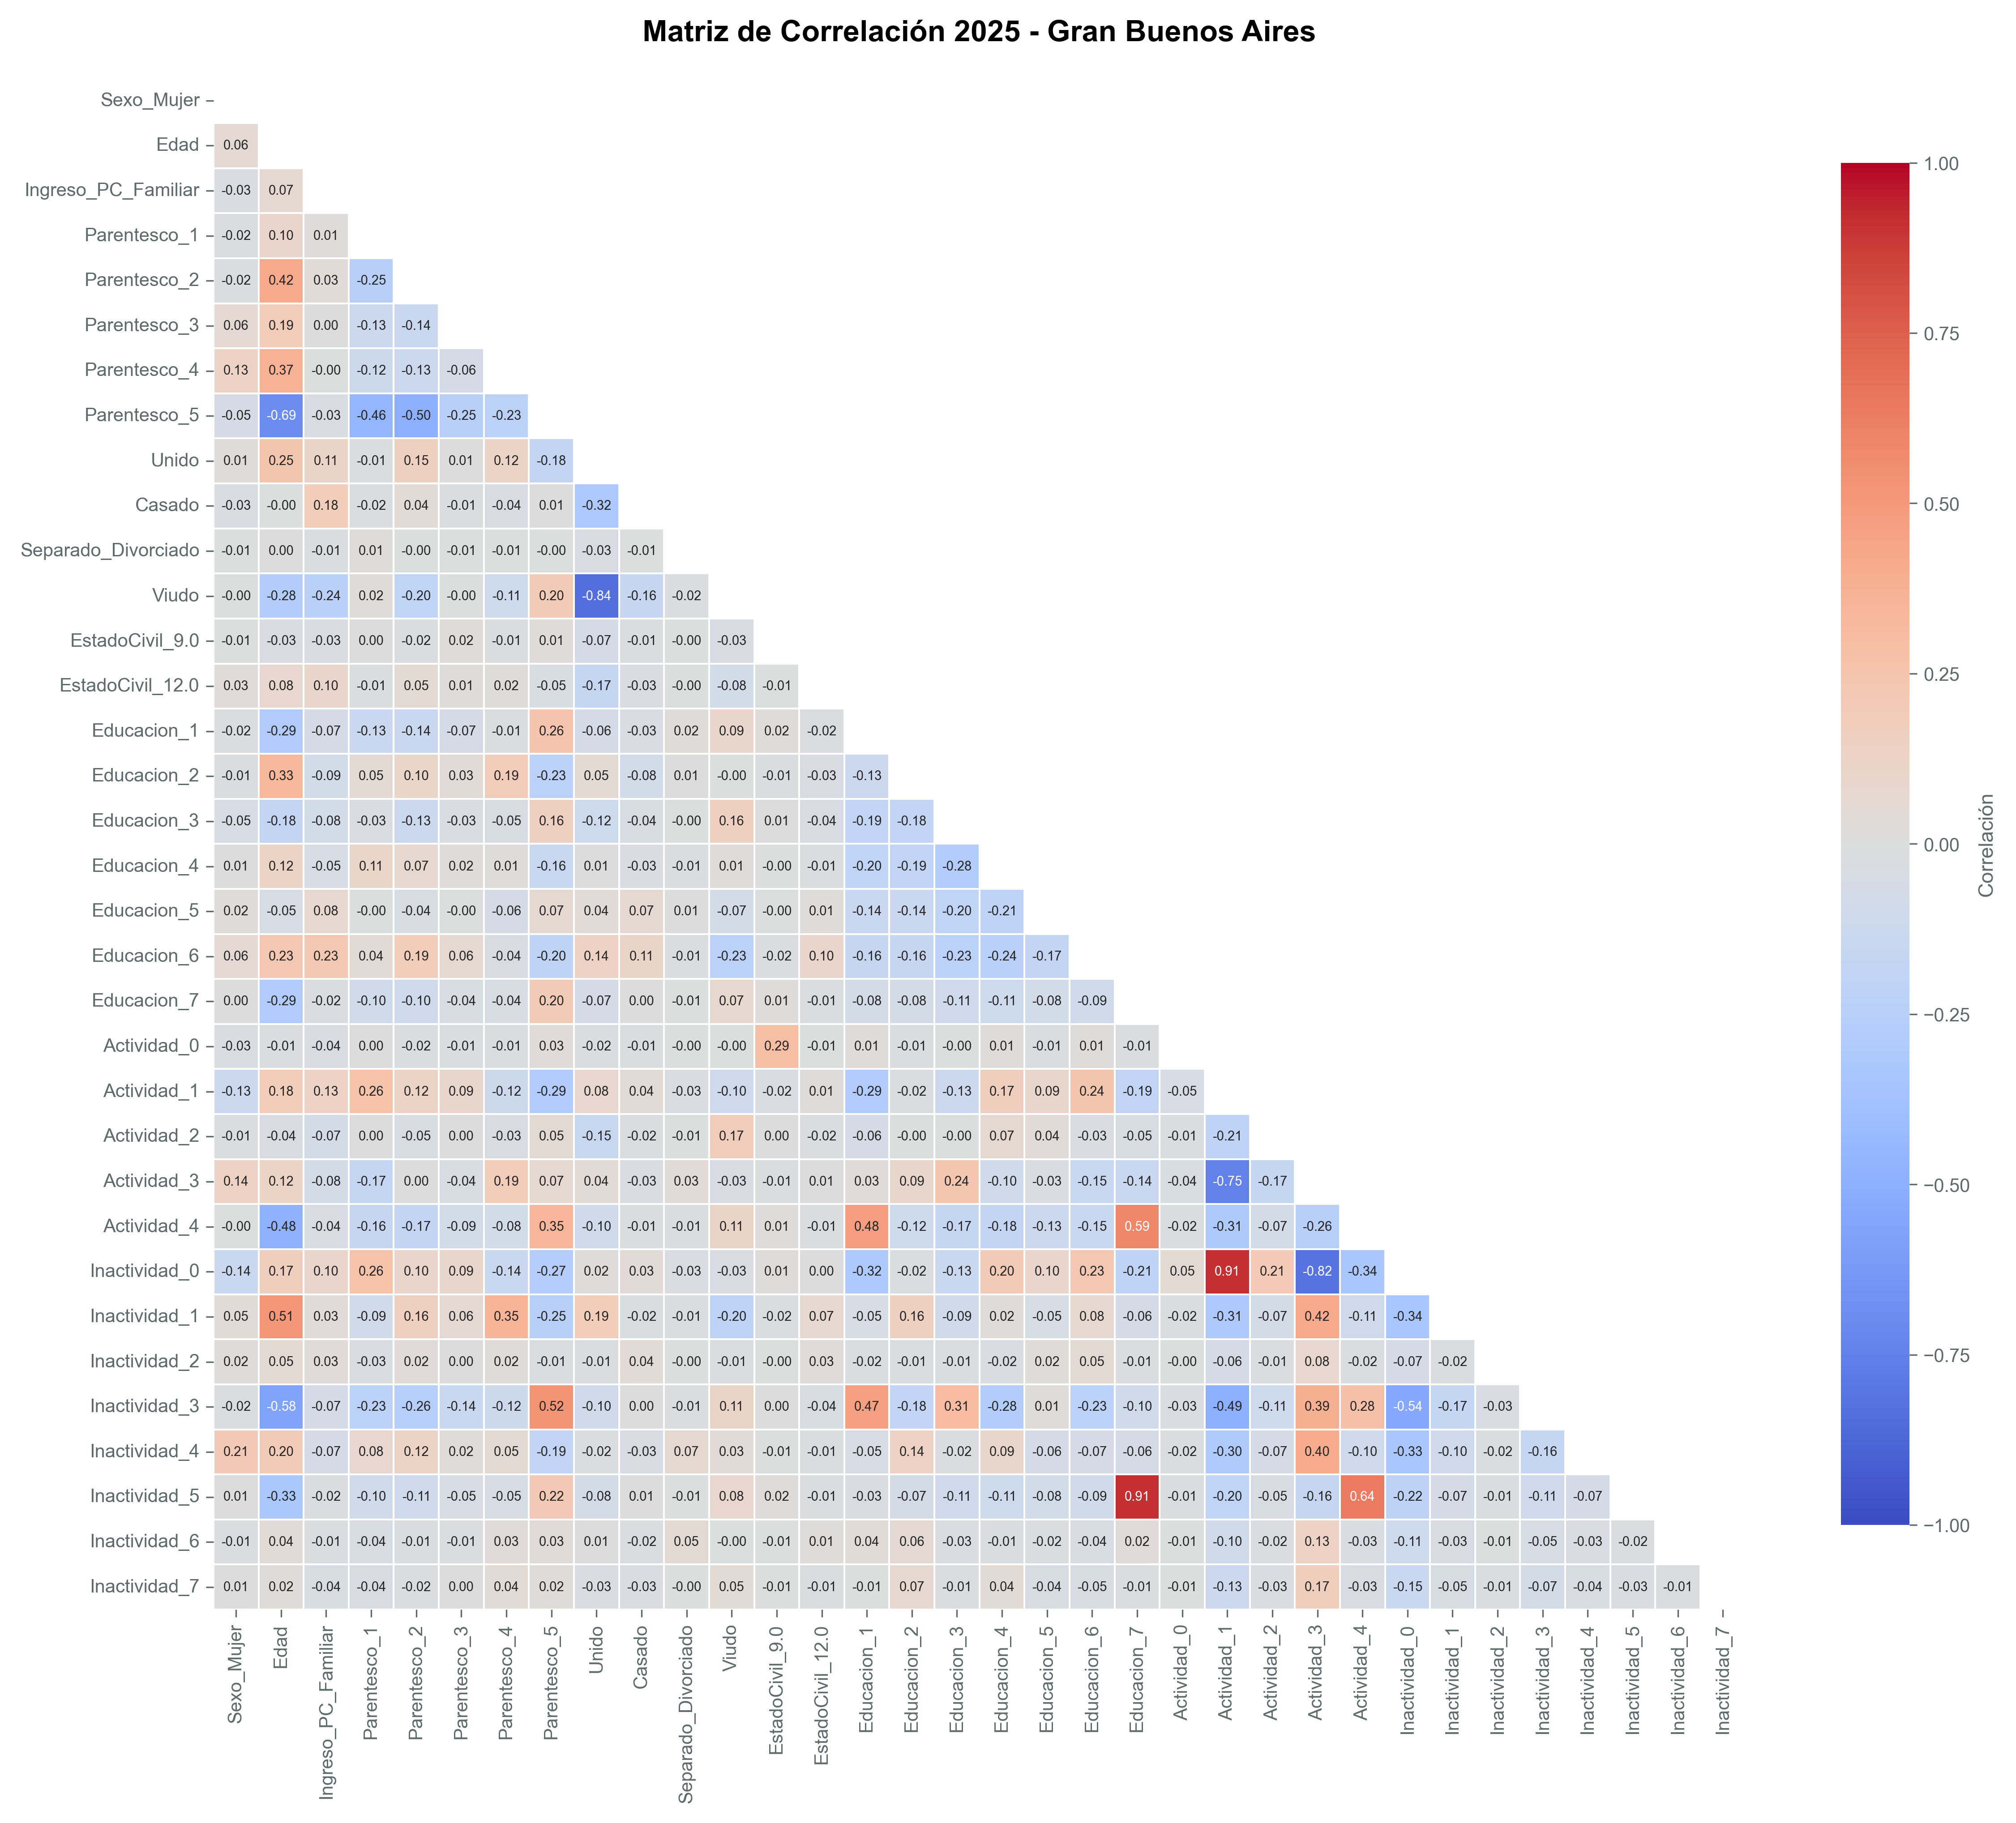
\includegraphics[width=0.75\textwidth]{../graficos/matriz_correlacion_2025.png}
    \caption{Matriz de correlación 2025 --- Gran Buenos Aires}
    \label{fig:corr2025}
\end{figure}

\begin{figure}[htb!]
    \centering
    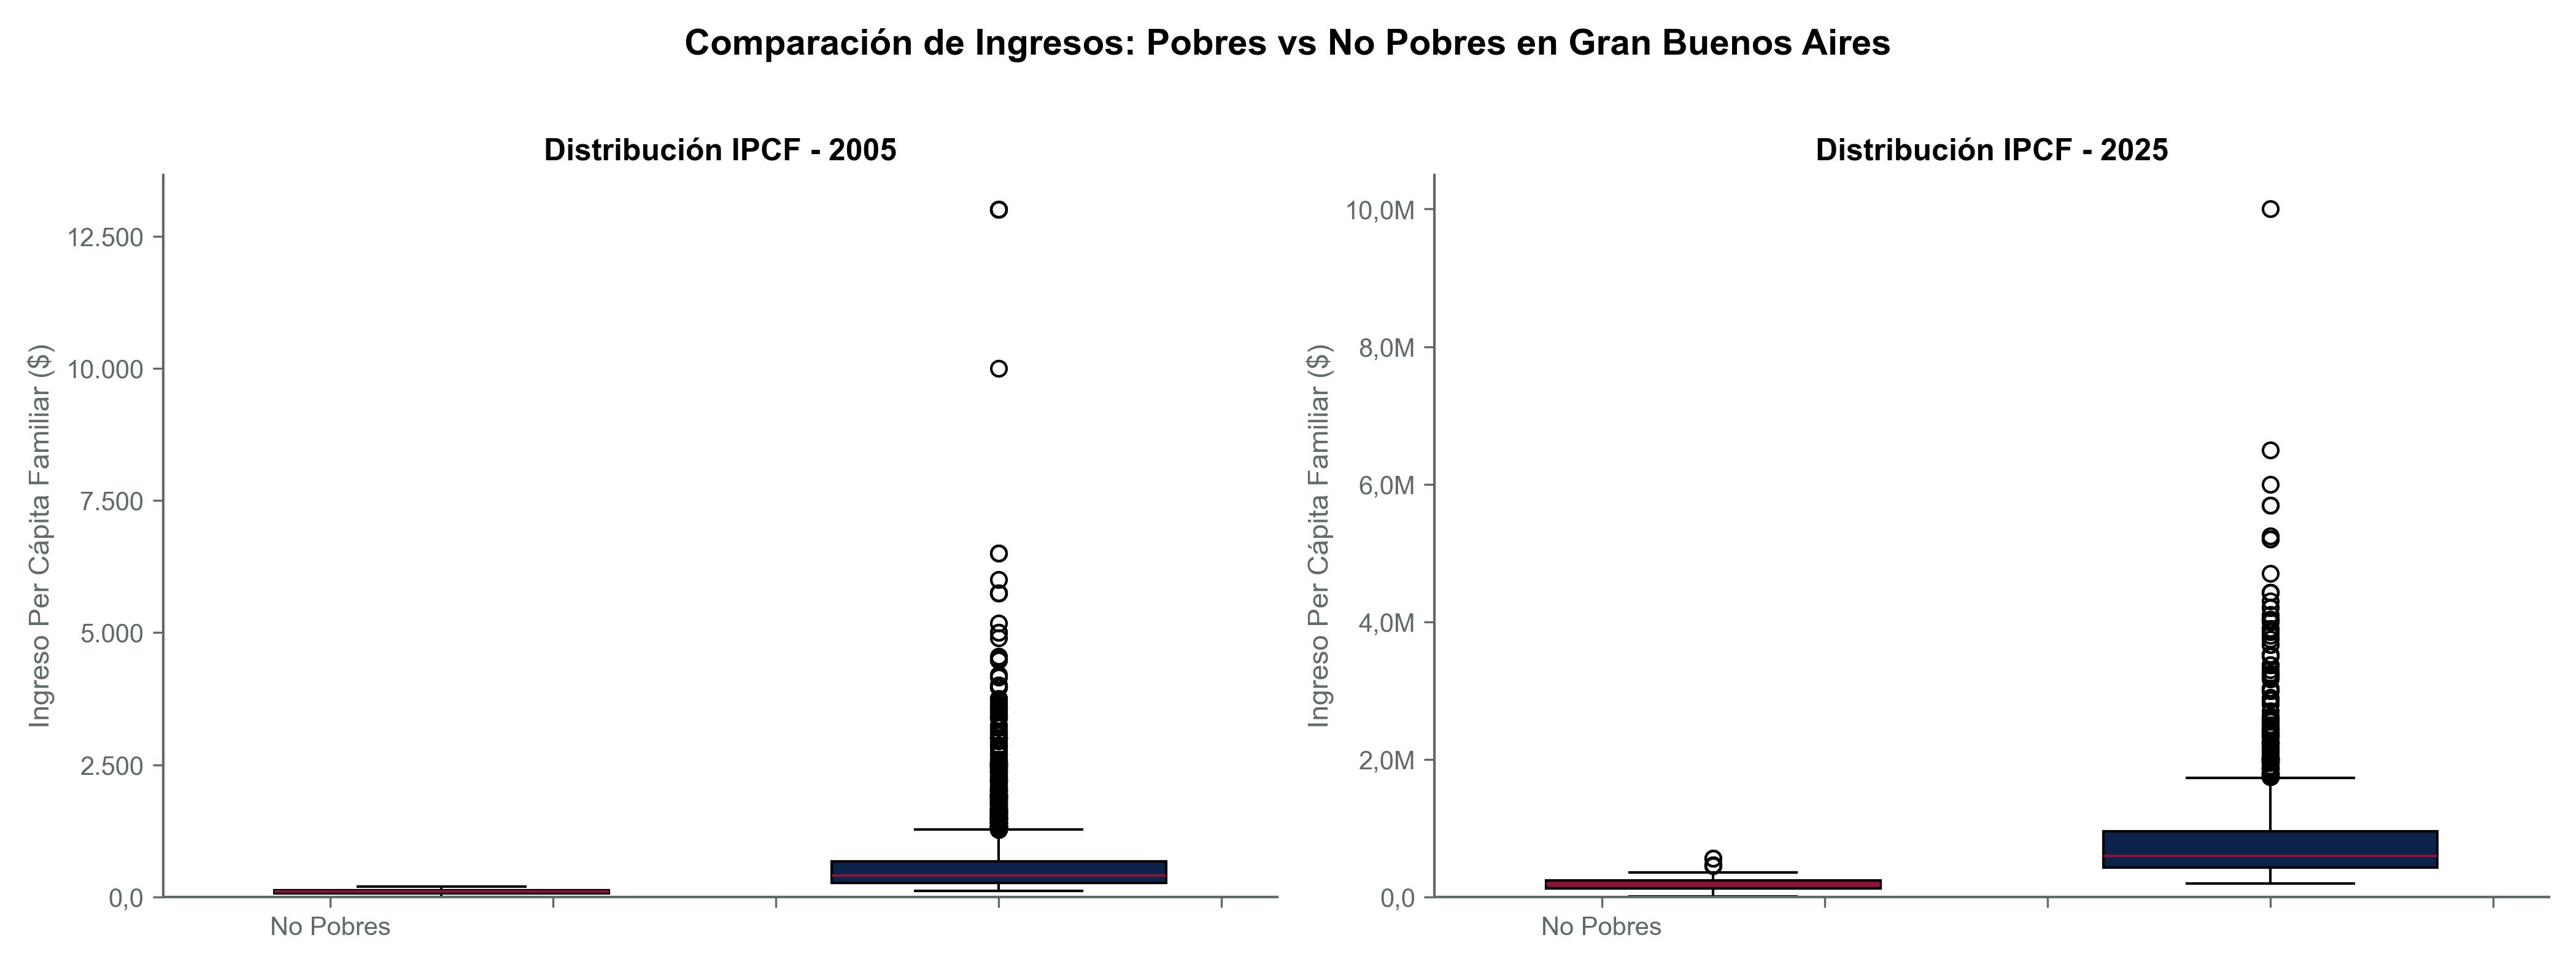
\includegraphics[width=\textwidth]{../graficos/distribucion_ipcf_pobres.png}
    \caption{Distribución del Ingreso Per Cápita Familiar: pobres vs no pobres}
    \label{fig:ipcf}
\end{figure}

\begin{figure}[htb!]
    \centering
    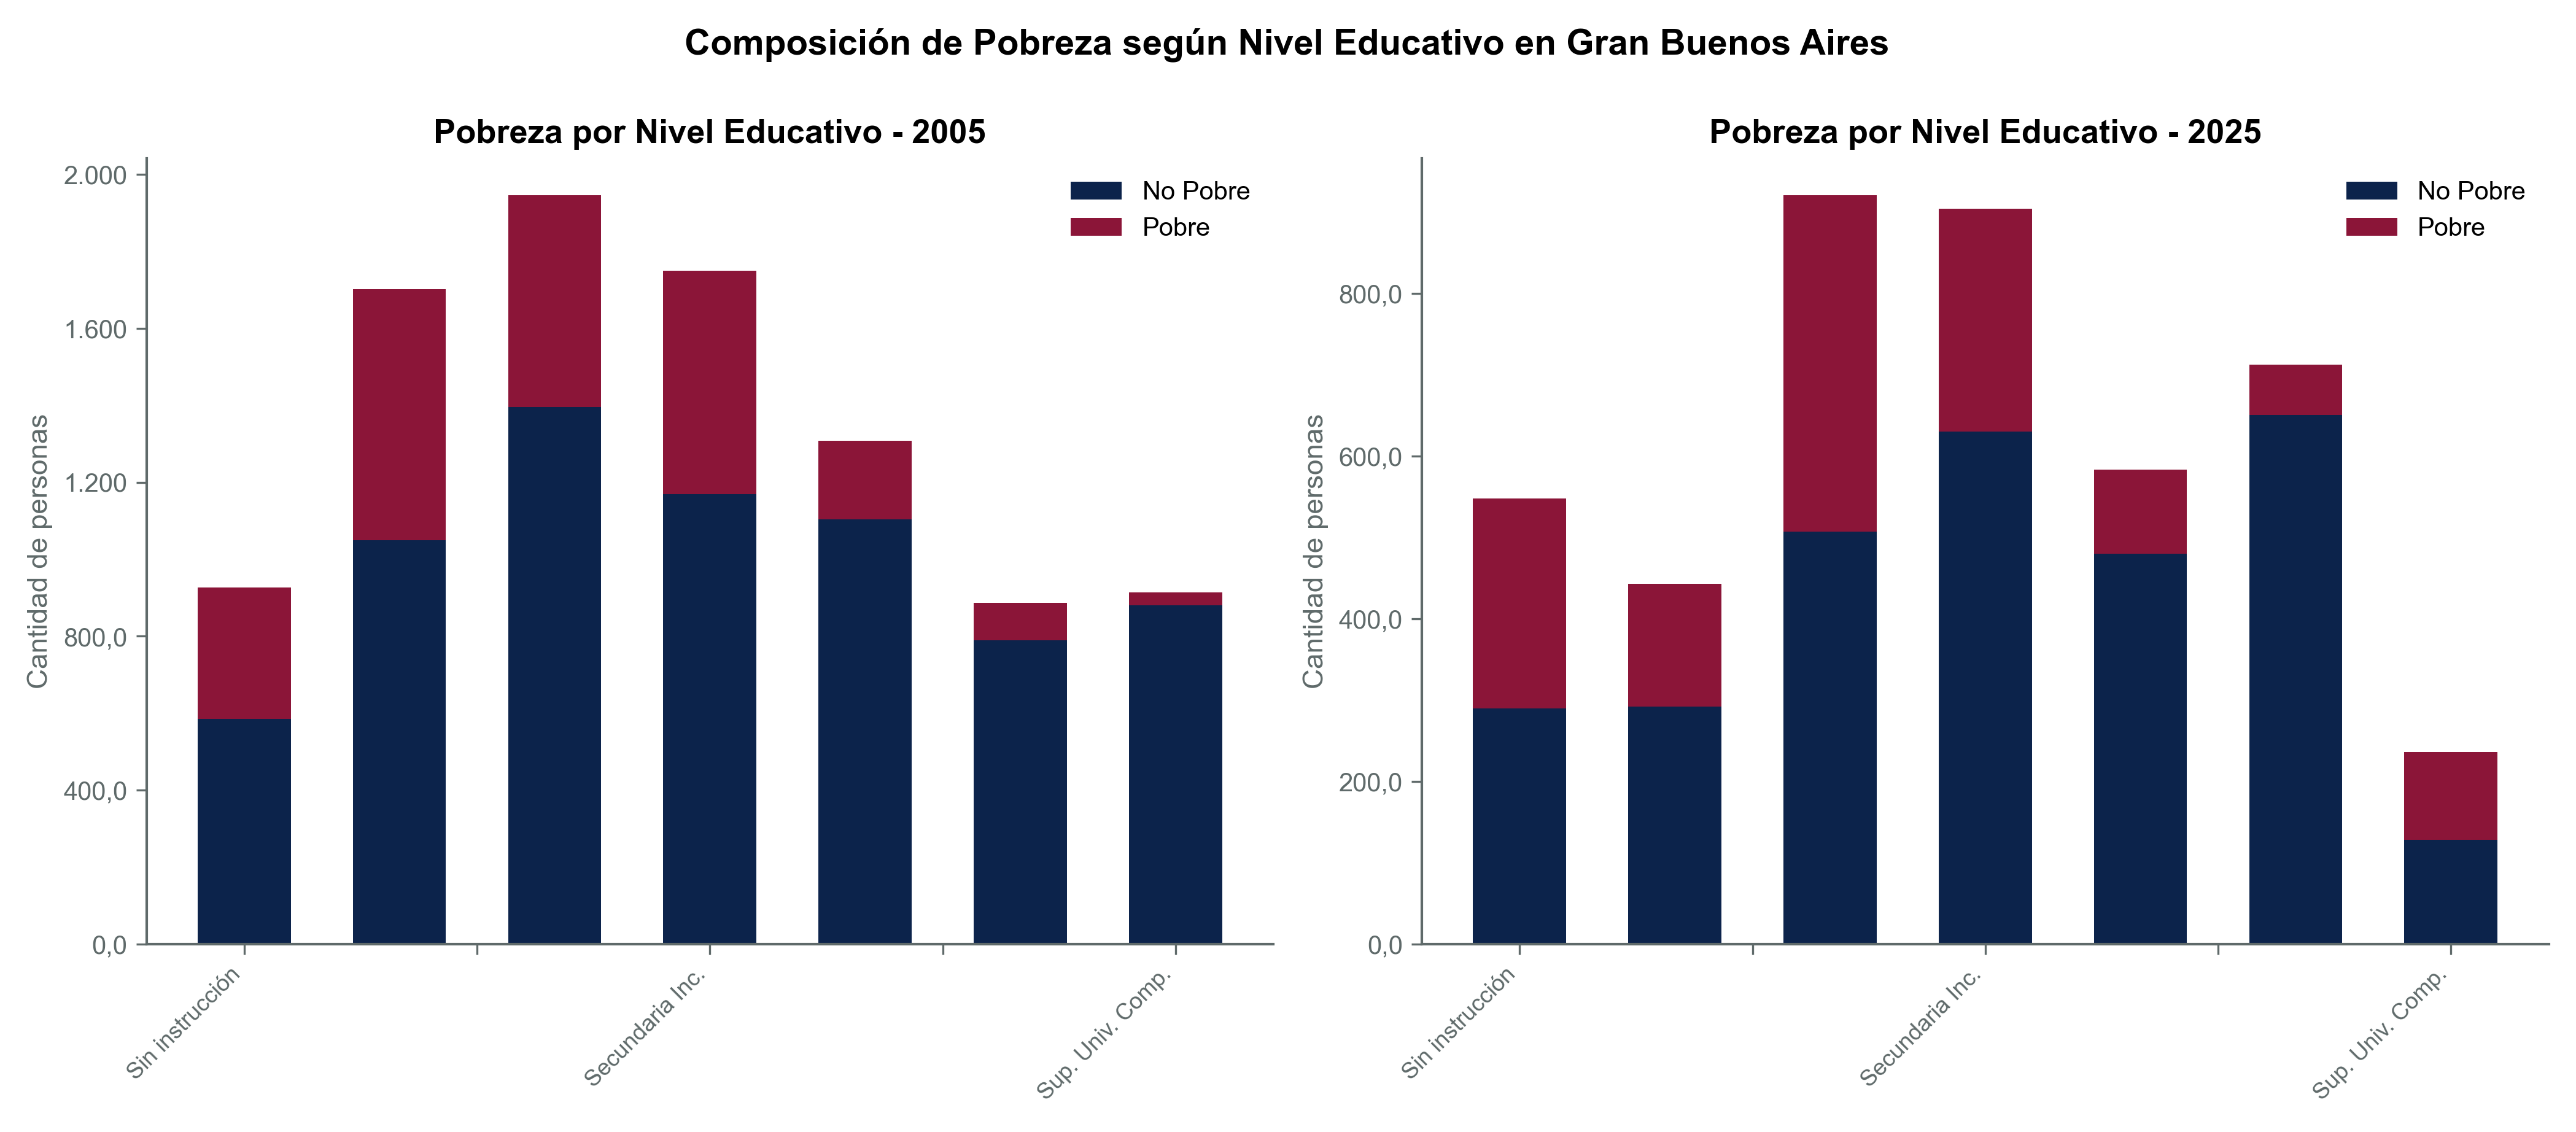
\includegraphics[width=\textwidth]{../graficos/pobreza_educacion.png}
    \caption{Composición de pobreza según nivel educativo en Gran Buenos Aires}
    \label{fig:educacion}
\end{figure}

\end{document}